\chapter{A VISUAL LANGUAGE MODEL FOR ESTIMATING OBJECT POSE AND STRUCTURE IN A GENERATIVE VISUAL DOMAIN}
\label{chapter:icra2011}

\section{Introduction}
\label{sec-ll1:introduction}

Human language is \emph{generative}:\footnote{We mean the Chomskyan sense of
  generative, not the sense in contrast to discriminative.
%
Indeed, while our domain is generative in the Chomskyan sense, our recognizer
uses a discriminative model.}  a small inventory of phonemes combine to yield a
large set of words and then this inventory of words combine to yield a larger
set of utterances.
%
Systems that process language must deal with the combinatorial nature of
generativity.
%
The probability of correct word recognition becomes fleetingly small with even
a slight probability for error in phoneme recognition and the probability of
determining the correct parse of an utterance becomes fleeting small with even
a slight probability for error in word recognition.
%
This is remedied with a \emph{language model}, a specification of which
combinations of phonemes constitute valid words and which combinations of
words constitute valid utterances.
%
Such a language model often takes the form of a \emph{grammar}.

The vast majority of computer-vision research in pose estimation and object
recognition deals with nongenerative collections of objects.
%
Such nongenerative collections require distinct models or exemplars for each
object (class) that varies greatly in shape, structure, or appearance.
%
We instead present an approach for doing pose estimation and structure
recognition in generative visual domains, analogous to the approach for human
language.
%
We illustrate this approach with the domain of \LincolnLog\ assemblies.
%
\LincolnLogs\ is a children's assembly toy with a small component inventory.
%
We limit this inventory to three component types: 1-notch, 2-notch, and 3-notch
logs.
%
These combine in myriad ways to yield a large set of assemblies.
%
We present low-level feature detectors that collect evidence for the components
in a fashion analogous to low-level feature detectors in speech recognizers.
%
But as in speech, the probability of correct recognition of an entire assembly
becomes fleetingly small with even a slight probability for error in log
recognition.
%
We remedy this with a \emph{visual language model} or a \emph{grammar} of
\LincolnLogs, a specification of which combinations of logs constitute valid
assemblies.

\begin{wrapfigure}[8]{r}{0.55\textwidth}
  \vspace*{-5ex}
  \centering
  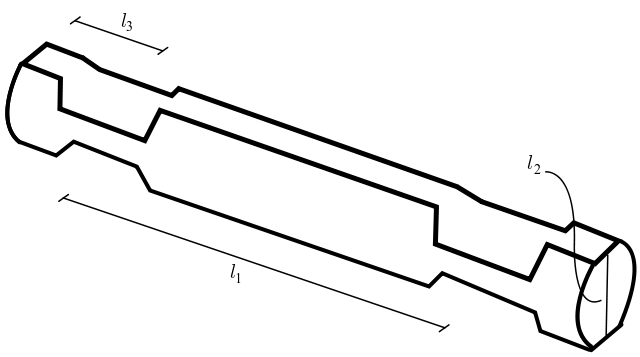
\includegraphics[width=0.55\textwidth]{images/log-parameters.png}
  \vspace*{-7ex}
  \caption{\small The 3D geometric shape parameters of \LincolnLogs.}
  \label{fig-ll1:logs}
\end{wrapfigure}
%
The analogy breaks down in two ways requiring novel methods.
%
First, most computer models of speech and language assume that the grammar is
context free.
%
This allows a top-down tree-structured generative process where the
generation of siblings is independent.
%
In contrast, the symbolic structure underlying \LincolnLog\ assemblies takes
the form of graphs with cycles and thus the visual language model is
context sensitive and is formulated as a stochastic constraint-satisfaction
problem.
%
Second, in language, all of the components are observable; at least in
principle, one can obtain perceptual evidence of each phoneme in a word and
each word in an utterance.
%
In contrast, visual domains exhibit \emph{occlusion}; it is almost always
necessary to determine object structure without perceptual evidence for all of
the components.
%
Our methods address both of these issues.
%
Our work builds upon the notion that scenes and objects are represented as
descriptions involving parts and spatial relations
\cite{Marr1978,Biederman1987,Wang2006,Zhu2006,Siskind2007,Zhu2007,Heitz2008,Lippow2008,Savova2008,
  Savova2009}, differing from prior work in the extreme degree of generativity
of the \LincolnLog\ domain.
%
None of this prior work focuses on domains that can generate as large a class
of distinct structures from as small a class of components.
%
Moreover, we focus on determining the precise pose and structure of an
assembly, including the 3D pose of each component, with sufficient accuracy to
support robotic manipulation and, in particular, the ability to robotically
construct a symbolically precise replicate of a structure from a single image.

\LincolnLog\ structures are composed out of a small inventory of components,
namely 1-notch, 2-notch, and 3-notch logs.
%
As shown in Fig.~\ref{fig-ll1:logs}, such logs are characterized by a small number
of shape parameters: the inter-notch distance~$l_1$, the log diameter~$l_2$, and
the distance~$l_3$ from a log end to the closest notch center.
%
Valid structures contain logs arranged so that their notches are aligned and
their medial axes are parallel to the work surface.
%
Thus valid structures have logs on alternating layers~$j$ at
height $l_2(j+0.5)$ oriented along one of two orthogonal sets of parallel lines
spaced equally with horizontal distance~$l_1$.
%
The lines for even layers are mutually parallel, the lines for odd layers are
mutually parallel, and the projections of a line from an even layer and an odd
layer onto the work surface are perpendicular.
%
We refer to this set of lines as the \defoccur{grid} (see Fig.~\ref{fig-ll1:pose}).
%
This grid imposes a symbolic structure on the \LincolnLog\ assembly.
%
Symbolic grid coordinates $(i,j,k)$ map to metric camera-relative
coordinates $(x,y,z)$ by the parameters~$l_1$, $l_2$, and~$l_3$ together with
the structure pose: the transformation from the grid coordinate system to the
camera coordinate system.
%
Estimating the structure of a \LincolnLog\ assembly thus reduces to two phases:
estimating the structure pose (section~\ref{sec-ll1:pose}) and determining the
log occupancy at each symbolic grid position (section~\ref{sec-ll1:occupancy}).

\section{Estimating the structure pose}
\label{sec-ll1:pose}

Before beginning these two phases, we first compute a mask that separates the
\LincolnLog\ structure in the image foreground from the background.
%
We manually collect 20--30 image segments of \LincolnLog\ components and compute
the mean~$\mu$ and covariance~$\Sigma$ of the pixel values in these segments in
a five-dimensional color space UVHSI.\@
%
We then derive a mask~$M$ from an input image~$I$ containing those pixels~$p$
with values whose Mahalanobis distance from~$\mu$ is less than or equal to a
threshold~$t$:
%
\[M_p =
\begin{cases}
  1 & \norm{C(I_p) - \mu}_{\Sigma}\leq t\\
  0 & \textrm{otherwise}\\
\end{cases}\]
%
where~$C$ denotes the map from input pixel values to UVHSI.\@

Nominally, the structure pose contains six degrees of freedom corresponding to
translation and rotation about each axis.
%
To simplify, we assume that the structure rests on the horizontal work surface.
%
Thus we fix vertical translation, roll around the camera axis, and pitch around
the horizontal axis perpendicular to the camera axis to be zero, leaving only
three free parameters: horizontal translation of the structure along the work
surface and yaw around the vertical axis.
%
To resolve the periodic translation ambiguity in the symbolic grid coordinate
system, we assume that the minimum occupied~$i$, $j$, and~$k$ values are
zero.
%
We further assume that we know the symbolic grid size: the maximum
occupied~$i$, $j$, and~$k$ values.

Images of \LincolnLog\ assemblies contain a predominance of straight edges that
result from log edges.
%
Given this, we estimate the structure pose in a two-step process.
%
We first find the pose~$p$ that maximizes the coincidence between the
set~$L(p)$ of projected grid lines~$l_g$ and the set~$L_I$ of image-edge
line segments~$l_i$:
%
\[\argmin_p\sum_{l_i\in L_I,l_g\in L(p)}\norm{l_i,l_g}\]
%
where $\norm{l_i,l_g}$ denotes the Euclidean distance between the midpoint of a
line segment and its closest point on a line, weighted by the disparity in
orientation between the line and the line-segment.
%
We then refine this pose estimate by maximizing the coincidence between
projected grid lines and the set~$P_I$ of image edge points~$p_i$:
%
\[\argmin_p\min_{p_i \in P_I,l_g \in L(p)}\norm{p_i,l_g}\]
%
where $\norm{p_i,l_g}$ denotes the Euclidean distance between a point and the
closest point on the line.
%
We use a soft $\min$ function \cite{Smale1986,Chen1993,Kanzow1996} when
computing the latter with gradient-based methods (reverse-mode automatic
differentiation \cite{Speelpenning1980}).

% parameters: Canny edge detector and Khoros line finder
% parameters: lower bound size
%
To obtain~$L_I$, we apply a Canny edge detector \cite{Canny1986} together with
the \Khoros\ line finder \cite{Konstantinides1994} to extract linear edge
segments from the input image, discarding short segments and those that do not
lie wholly within the mask region defined by~$M$.
%
% parameters: how many bins
%
We then select the edge segments corresponding to the two most prominent edge
orientations, by placing the segments into bins according to their orientation
and selecting the edge segments in the two largest bins.
%
% parameters: of Phase Congruency
%
To obtain~$P_I$, we apply Phase Congruency \cite{Kovesi1999} to the input
image~$I$ to compute the orientation image~$O(I)$.
%
Each pixel in~$O(I)$ contains a quantized orientation.
%
We chose~$P_I$ to be those pixels whose quantized orientation is closest to the
mean edge-segment orientations of the above two largest bins.

This two-step process offers several advantages.
%
The first step converges quickly but exhibits error in the recovered prominent
edge orientations.
%
The second step estimates pose more accurately (typically within~5mm translation
and~2$^{\circ}$ rotation), but only with close initial estimates, such as those
provided by the first step.

Fig.~\ref{fig-ll1:pose} illustrates successful pose estimation of several
\LincolnLog\ structures.
%
Note that we estimate the pose of a target object from a single image without
any knowledge of the specific 3D shape or structure of that object, without any
prior training images of that object in different poses, using only generic
information from the domain, namely that the object is a valid \LincolnLog\
assembly.

\begin{figure}
\centering
\begin{tabular}{@{}c@{\hspace*{4pt}}c@{}}
  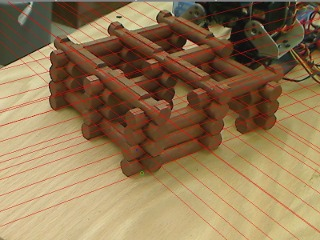
\includegraphics[width=0.48\textwidth]{images/pose1-cut.jpg}
  &
  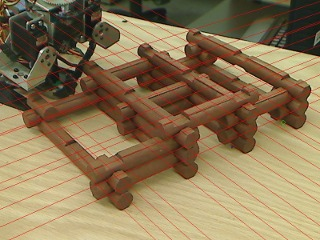
\includegraphics[width=0.48\textwidth]{images/pose2-cut.jpg}
\end{tabular}
%
\caption{\small Estimating the pose of an arbitrary \LincolnLog\ assembly and
  the symbolic grid thus imposed on the assembly.}
%
\label{fig-ll1:pose}
\end{figure}

\section{Determining the log occupancy at each symbolic grid position}
\label{sec-ll1:occupancy}

The symbolic grid positions~$q=(i,j,k)$ refer to points along log medial axes
at notch centers.
%
Each such grid position may be either unoccupied, denoted by~$\emptyset$, or
occupied with the~$n^{\textrm{th}}$ notch, counting from zero, of a log
with~$m$ notches, denoted by $(m,n)$.
%
For each grid position we wish to determine its occupancy, one of seven
possibilities: $\emptyset$, $(1,0)$, $(2,0)$, $(2,1)$, $(3,0)$, $(3,1)$, and
$(3,2)$.
%
We construct a discrete random variable~$Z_q$ for each grid position~$q$ that
ranges over these seven possibilities.

\begin{figure}
\centering
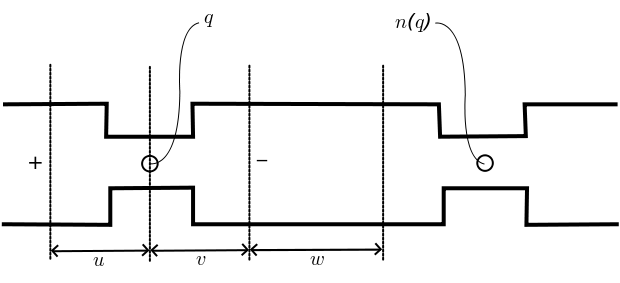
\includegraphics[width=0.7\textwidth]{images/random-variables.png}
%
\vskip -18px
\caption{\small The random variables~$Z^+_q$ and~$Z^-_q$ that correspond to log
  ends for grid position~$q$ and the random variables~$Z^u_q$, $Z^v_q$,
  and~$Z^w_q$ that correspond to log segments.}
%
\label{fig-ll1:endsandsegs}
\vskip -15px
\end{figure}

We determine several forms of image evidence for the log occupancy of a given
grid position.
%
\LincolnLogs, being cylindrical structures, generate two predominant image
features: ellipses that result from the perspective projection of circular log
ends and line segments that result from the perspective projection of
cylindrical walls.
%
We refer to the former as \defoccur{log ends} and the latter as \defoccur{log
  segments}.
%
Log ends can potentially appear only at distance~$\pm l_3$ from grid positions
along the direction for the layer of that grid position.
%
We construct boolean random variables~$Z^+_q$ and~$Z^-_q$ to encode the
presence or absence of a log end at such positions.
%
There are two kinds of log segments: ones corresponding to~$l_1$ and ones
corresponding to~$l_3$.
%
Given this, we construct three boolean random variables~$Z^u_q$, $Z^v_q$,
and~$Z^w_q$ for each grid position~$q$ that encode the presence or absence of
log segments for the bottoms of logs, \ie\ log segments between a grid position
and the adjacent grid position below.
%
$Z^u_q$~and~$Z^v_q$ encode the presence or absence of a log segment of
length~$l_3$ behind and ahead of~$q$ respectively, along the direction for the
layer of~$q$ while~$Z^w_q$ encodes the presence or absence of a log segment of
length $l_1-2l_3$ between grid positions along the same layer.
%
Fig.~\ref{fig-ll1:endsandsegs} depicts the log ends and log segments that
correspond to a given grid position as described above.

We formulate a stochastic constraint-satisfaction problem
(CSP \cite{Lauriere1978}) over these random variables.
%
The constraints encode the validity of an assembly.
%
We refer to these constraints as the \defoccur{grammar} of
\LincolnLogs\ (section~\ref{sec-ll1:grammar}).
%
We take image evidence to impose priors on the variables~$Z^+_q$, $Z^-_q$,
$Z^u_q$, $Z^v_q$, and~$Z^w_q$ (sections~\ref{sec-ll1:evidence}
and~\ref{sec-ll1:mapping}) and solve this stochastic CSP to perform structure
estimation (section~\ref{sec-ll1:structure}).

\subsection{Evidence for the presence or absence of logs}
\label{sec-ll1:evidence}

\begin{wrapfigure}[9]{r}{0.48\textwidth}
\centering
\vskip -20px
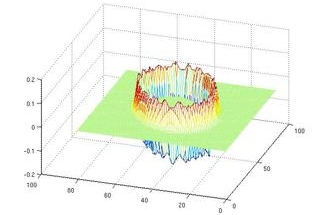
\includegraphics[width=0.48\textwidth]{images/ellipse-filter-small.jpg}
\vskip -12px
\caption{\small Elliptical edge filter for detecting log ends}
\label{fig-ll1:efilter}
\end{wrapfigure}
%
Given the pose~$p$, a log end present as the result of~$Z^+_q$ or~$Z^-_q$ being
true will manifest as an ellipse of known shape, size, and position in the
image.
%
We use $x^+(p,q)$, $y^+(p,q)$, $a^+(p,q)$, $b^+(p,q)$, and $\theta^+(p,q)$ to
denote the parameters (center, lengths of major and minor axes, and orientation
of major axis) of an ellipse that would manifest from~$Z^+_q$ and similarly
for~$Z^-_q$.
%
We find these parameters by a least-squares fit of 20 equally spaced 3D points
on the log end projected to the image.
%
The 3D points can be determined in closed form from the grid position~$q$ and
the parameters~$l_1$, $l_2$, and~$l_3$.
%
% parameters: r and \sigma
%
We then construct an indicator function~$f(x,y)$ with the value~1 for
points~$(x,y)$ inside the ellipse and the value~0 for points outside the
ellipse and convolve this with a Laplacian of a Gaussian filter,
$\mathrm{LoG}(r,\sigma)$, to obtain an elliptical edge filter~$E(x,y,a,b,\theta)$
(Fig.~\ref{fig-ll1:efilter}).
%
Nominally, a high response to this filter applied to an image correlates with
the presence of an elliptical feature with parameters $x$, $y$, $a$, $b$, and
$\theta$.
%
To provide robustness in the face of inaccurate pose estimation, we compute the
maximal filter response in a 5-dimensional region centered on $x$, $y$, $a$,
$b$, and $\theta$ derived by perturbing each axis a small amount.

Similarly, given the pose~$p$, a log segment present as the result of~$Z^u_q$,
$Z^v_q$, or~$Z^w_q$ being true will manifest as a line segment between known
image points.
%
We denote the points for~$Z^u_q$ as $(x^u_1(p,q),y^u_1(p,q))$ and
$(x^u_2(p,q),y^u_2(p,q))$ and similarly for~$Z^v_q$ and~$Z^w_q$.
%
These image points can be determined in closed form by projecting the 3D points
derived from the pose~$p$, the grid position~$q$, and the
parameters~$l_1$, $l_2$, and~$l_3$.

In principle, we could use a similar filter method to determine evidence for
log segments.
%
However, log ends usually yield highly pronounced edges because logs are never
stacked horizontally end to end.
%
Log are often stacked vertically and the log segments between two such
vertically stacked logs would yield less-pronounced edges.
%
Thus we use a more sensitive method to determine evidence for log segments.
%
Given the pose~$p$ of the structure, we recompute the prominent edge
orientations~$o_1$ and~$o_2$ using the methods from section~\ref{sec-ll1:pose}
(this time applied to the output of the second step of pose estimation, not the
first, to give a more accurate estimate of these orientations).
%
For each prominent orientation~$o$, we compute the disparity between~$o$
and~$O(I)$ at each pixel, compute the prominence at each pixel by attenuating
the disparity, and scale the energy image, $E(I)$, by this prominence:
%
$W(I,o)=E(I)\circ\cos^2(O(I)-o)$.
%
This constitutes a graded edge map for edges with orientation~$o$.
%
% parameters: threshold
%
We search a rectangular region in~$W(I,o)$, after thresholding, for the longest
line segment.
%
% parameters: dilation
%
The search region corresponds to a dilation of the rectangle bounded by the
endpoints of the target log segment.
%
The length of the longest line segment found correlates with the presence of the
target log segment.

\subsection{Mapping evidence to priors}
\label{sec-ll1:mapping}
%
We train a mapping function from evidence to priors for the log-segment and
log-end evidence functions respectively on a set of~30 images annotated with
ground truth, \ie\ true positives and true negatives, along with occlusion.
%
For each evidence function, we bin their respective raw, real-valued responses
into~20 bins and annotate each bin with the percentage of responses that are
true positives and the central response value for that bin.
%
The annotated bins correspond to a discrete sequence of impulses with impulse
magnitude representing the percentage of true positives for the central response
value.
%
We then employ a weighted linear interpolation function between impulses to
provide the mapping function.
%
The weighting factor~$e$ typically takes the form of a real value $e\in(0,1)$.

\subsection{The grammar of Lincoln Logs}
\label{sec-ll1:grammar}

% needs work: reusing b, n, and p

We refer to the adjacent grid position below~$q$ as~$b(q)$, the adjacent grid
position further from the origin along the direction of the grid lines for the
layer of~$q$ as~$n(q)$, and the adjacent grid position closer to the origin
along the direction of the grid lines for the layer of~$q$ as~$p(q)$.
%
Ignoring boundary conditions at the perimeter of the grid, the grammar of
\LincolnLogs\ can be formulated as the following constraints:
%
\begin{compactenum}[a)]
%
\item 2-notch logs occupy two adjacent grid points
%
\label{constraintA}
%
\begin{displaymath}
Z_q=(2,0)\leftrightarrow Z_{n(q)}=(2,1)
\end{displaymath}
%
\item 3-notch logs occupy three adjacent grid points
%
\label{constraintB}
%
\begin{displaymath}
\begin{array}{r@{\;}c@{\;}l}
Z_q=(3,0)&\leftrightarrow&Z_{n(q)}=(3,1)\\
Z_q=(3,0)&\leftrightarrow&Z_{n(n(q))}=(3,2)\\
Z_{n(q)}=(3,1)&\leftrightarrow&Z_{n(n(q))}=(3,2)
\end{array}
\end{displaymath}
%
\item 1- and 2-notch logs must be supported at all notches
%
\label{constraintC}
%
\begin{displaymath}
Z_q\in\theset{(1,0),(2,0),(2,1)}\rightarrow Z_{b(q)}\not=\emptyset
\end{displaymath}
%
\item 3-notch logs must be supported in at least 2 notches
%
\label{constraintD}
%
\begin{displaymath}
Z_q=(3,0)\rightarrow
\left(\begin{array}{l}
\left(Z_{b(q)}\not=\emptyset\wedge Z_{b(n(q))}\not=\emptyset\right)\vee\\
\left(Z_{b(q)}\not=\emptyset\wedge Z_{b(n(n(q)))}\not=\emptyset\right)\vee\\
\left(Z_{b(n(q))}\not=\emptyset\wedge Z_{b(n(n(q)))}\not=\emptyset\right)
\end{array}\right)
\end{displaymath}
%
\item log ends must be at the ends of logs
%
\label{constraintE}
%
\begin{displaymath}
\begin{array}{r@{\;}c@{\;}l}
Z^-_q&\leftrightarrow&Z_q\in\theset{(1,0),(2,0),(3,0)}\\
Z^+_q&\leftrightarrow&Z_q\in\theset{(1,0),(2,1),(3,2)}
\end{array}
\end{displaymath}
%
\item short log segments indicate occupancy above or below
%
\label{constraintF}
%
\begin{displaymath}
\begin{array}{r@{\;}c@{\;}l}
Z^u_q&\leftrightarrow&
\left(Z_q\not=\emptyset\vee Z_{b(b(q))}\not=\emptyset\right)\\
Z^v_q&\leftrightarrow&
\left(Z_q\not=\emptyset\vee Z_{b(b(q))}\not=\emptyset\right)
\end{array}
\end{displaymath}
%
\item long log segments indicate presence of a multi-notch log above or below
%
\label{constraintG}
%
\begin{displaymath}
Z^w_q\leftrightarrow
\left(\begin{array}{l}
\left(\begin{array}{l}
    Z_q\in\theset{(2,0),(3,0),(3,1)}\wedge\\
    Z_{n(q)}\in\theset{(2,1),(3,1),(3,2)}\\
\end{array}\right)\vee\\
\left(\begin{array}{l}
    Z_{b(b(q))}\in\theset{(2,0),(3,0),(3,1)}\wedge\\
    Z_{b(b(n(q)))}\in\theset{(2,1),(3,1),(3,2)}
\end{array}\right)
\end{array}\right)
\end{displaymath}
\end{compactenum}
%
To handle the boundary conditions, we stipulate that the grid positions beyond
the perimeter are unoccupied, enforce the support requirement (constraints
\ref{constraintC}--\ref{constraintD}) only at layers above the lowest layer,
and enforce log-segment constraints (\ref{constraintF}--\ref{constraintG}) for
the layer above the top of the structure.

\subsection{Structure estimation}
\label{sec-ll1:structure}
%
To perform structure estimation we first establish priors over the random
variables~$Z^+_q$ and~$Z^-_q$ that correspond to log ends and the random
variables~$Z^u_q$, $Z^v_q$, and~$Z^w_q$ that correspond to log segments using
image evidence and establish a uniform prior over the random variables~$Z_q$.
%
This induces a probability distribution over the joint support of these random
variables.
%
We then marginalize the random variables that correspond to log ends and log
segments and condition this marginal distribution on the language model~$\Phi$.
%
Finally, we compute the assignment to the random variables~$Z_q$ that maximizes
this conditional marginal probability.
%
\begin{displaymath}
\argmax_{\mathbf{Z}}
\sum_{\substack{\mathbf{Z}^+,\mathbf{Z}^-,\mathbf{Z}^u,\mathbf{Z}^v,\mathbf{Z}^w\\
    \Phi\left[\mathbf{Z},\mathbf{Z}^+,\mathbf{Z}^-,\mathbf{Z}^u,\mathbf{Z}^v,\mathbf{Z}^w\right]}}
\Pr\left(\bigwedge_q Z_q,Z^+_q,Z^-_q,Z^u_q,Z^v_q,Z^w_q\right)
\end{displaymath}
%
To speed up the conditional marginalization process, we prune assignments to
the random variables that violate the grammar~$\Phi$ using arc consistency
\cite{Mackworth1977}.
%
To speed up the maximization process, we use a branch-and-bound algorithm
\cite{Land1960} that maintains upper and lower bounds on the maximal
conditional marginal probability.
%
Without both of these, structure estimation would be intractable.

An alternate method to perform structure optimization is to establish the same
priors over the random variables that correspond to log ends and log segments
but parametrize the priors over the random variables~$Z_q$.
%
We then marginalize over all random variables, computing this marginal
probability over the parameterized priors for the random variables~$Z_q$.
%
We then search over this parameter space for the distributions over the random
variables~$Z_q$ that maximize this marginal probability.
%
We do this using the reduced-gradient optimization algorithm
\cite{Wolfe1962,Wolfe1967} where the gradients are calculated using
reverse-mode AD.\@
%
The linear constraints are used to constrain the parameters of the probability
distribution to be nonnegative and sum to one.
%
Ideally, we'd prefer to use the latter method exclusively, but the former
method is faster to compute for the relatively larger assemblies when compared
to the latter.

\subsection{Occlusion}
\label{sec-ll1:occlusion}

Nominally, with the above method, one derives evidence for the presence or
absence of log ends and log segments of the various kinds at every possible
grid position.
%
In other words, one uses image evidence to impose a prior on all of the random
variables~$Z^+_q$, $Z^-_q$, $Z^u_q$, $Z^v_q$, and~$Z^w_q$.
%
However, some of these log ends and log segments may be occluded.
%
If we \emph{know} that a log end or log segment is occluded then we ignore all
evidence for it from the image, giving it chance probability of being occupied.
%
With this, the grammar can often fill in the correct values of occluded random
variables for both log ends and log segments, and thus determine the correct
value for an occluded $Z_q$.
%
The question then arises: how does one determine whether a log end or log
segment is occluded?
%
We propose the following method.
%
One first assumes that all of the log ends and log segments on the frontal
faces of the grid are visible but all other log ends and log segments are
occluded.
%
One then performs structure estimation under this initial hypothesis.
%
With the recovered structure estimate, one determines log-end and log-segment
visibility by projective geometry given the known pose, and iterates this
process until convergence.
%
We have recently implemented this algorithm and expect to report on its
performance in the future.
%
All experiments reported in section~\ref{sec-ll1:results} were performed with
manual annotation of occlusion information.
%
Note that we only annotate for a given symbolic log-segment or log-end
\emph{position} whether or not it is \emph{visible}, \textbf{not} whether or
not that position is \emph{occupied} with a log segment or log end.
%
The latter is determined automatically.

\section{Experimental results}
\label{sec-ll1:results}
\addtolength{\textheight}{-0.32cm}

\begin{figure}
\centering
\hskip -10px
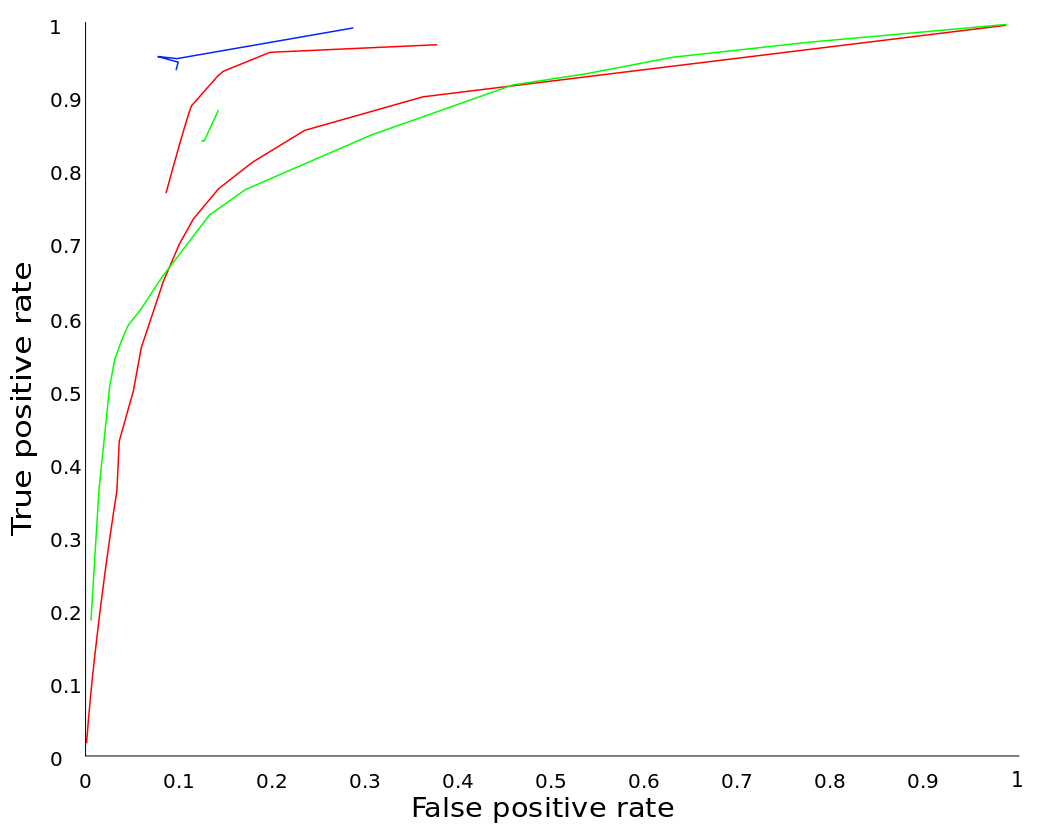
\includegraphics[width=1.0\textwidth]{images/graph.png}
\vskip -20px
%
\caption{\small ROC curves.
%
The lower green and red curves constitute the ROC for the log-end and
log-segment detectors respectively with varying thresholds~$t$ without the
grammar.
%
The upper green curve measures ROC for~$Z^+_q$ and~$Z^-_q$ under constraints
\ref{constraintA}--\ref{constraintE} varying the mapping from evidence to
priors.
%
The upper red curve measures ROC for~$Z^u_q$, $Z^v_q$, and~$Z^w_q$ under
constraints \ref{constraintA}--\ref{constraintD} and
\ref{constraintF}--\ref{constraintG} varying the mapping from evidence to
priors.
%
The blue curve measures ROC for~$Z^+_q$, $Z^-_q$, $Z^u_q$, $Z^v_q$, and~$Z^w_q$
under all constraints varying the mapping from evidence to priors.}
%
\label{fig-ll1:roc}
\vskip-3ex
\end{figure}

\begin{figure}
\centering
% \begin{tabular}{@{}c@{\hspace*{2pt}}c@{\hspace*{2pt}}c@{\hspace*{2pt}}c@{}}
% 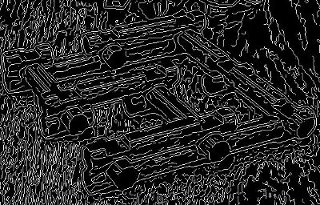
\includegraphics[width=0.25\textwidth]{images/1263244624-1500-matlab.jpeg}&
% 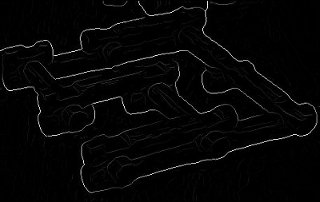
\includegraphics[width=0.25\textwidth]{images/1263244624-1500-pb.jpeg}&
% 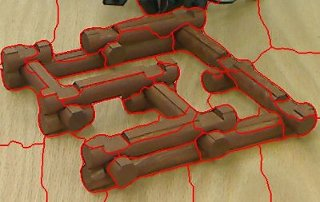
\includegraphics[width=0.25\textwidth]{images/1263244624-1500-ncuts.jpeg}&
% 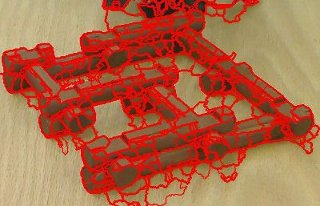
\includegraphics[width=0.25\textwidth]{images/1263244624-1500-mshift.jpeg}\\
% (a)&(b)&(c)&(d)
% \end{tabular}
\begin{tabular}{@{}c@{\hspace*{2pt}}c@{}}
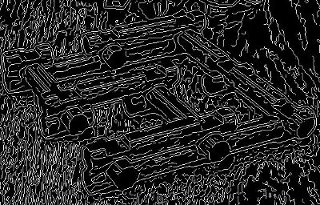
\includegraphics[height=0.215\textheight]{images/1263244624-1500-matlab.jpeg}&
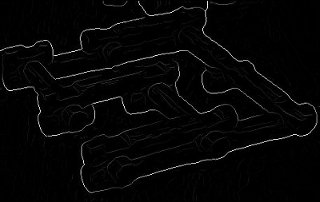
\includegraphics[height=0.215\textheight]{images/1263244624-1500-pb.jpeg}\\
(a)&(b)\\[1ex]
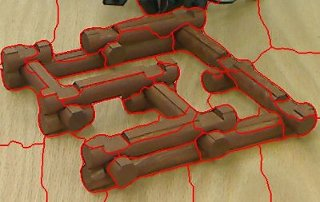
\includegraphics[height=0.215\textheight]{images/1263244624-1500-ncuts.jpeg}&
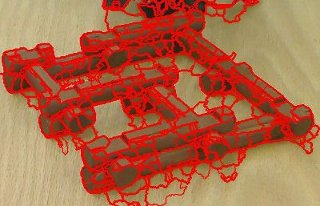
\includegraphics[height=0.215\textheight]{images/1263244624-1500-mshift.jpeg}\\
(c)&(d)
\end{tabular}
\vspace*{-4ex}
\caption{\small A comparison with a number of standard edge detectors and segmentation methods.
%
Neither (a)~\Matlab's Canny edge detector nor (b)~the \Pb\ edge detector reliably find edges separating adjacent logs or log ends.
%
Neither (c)~Normalized Cut nor (d)~Mean Shift segment out the log parts.}
%
\label{fig-ll1:comparison}
\end{figure}


\begin{figure}
\centering
\begin{tabular}{@{}c@{\hspace*{2pt}}c@{\hspace*{2pt}}c@{\hspace*{2pt}}c@{\hspace*{2pt}}c@{}}
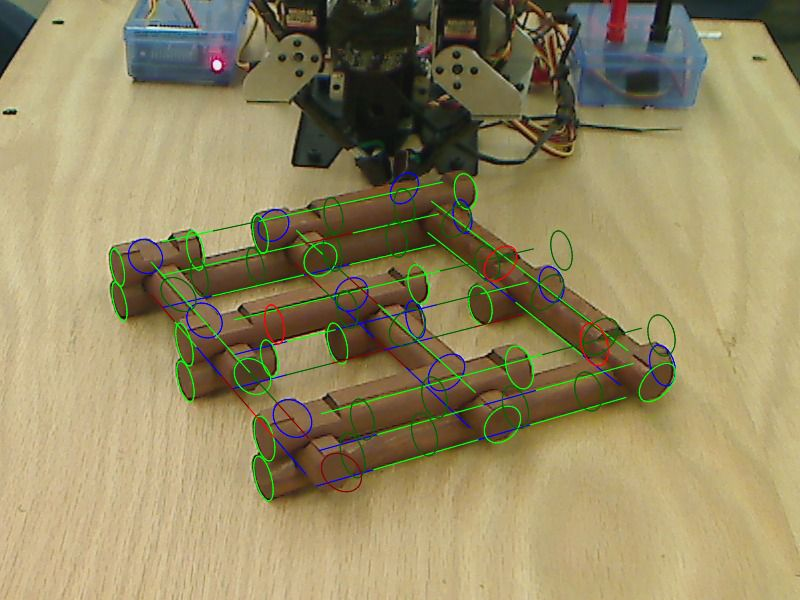
\includegraphics[width=0.195\textwidth]{images/1263244624-1500-0-raw.jpg}&
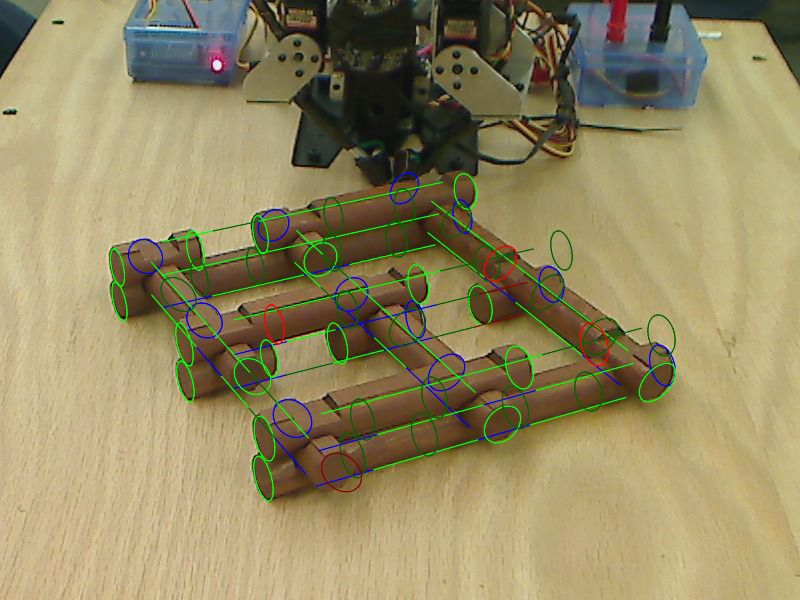
\includegraphics[width=0.195\textwidth]{images/1263244624-1500-0-segment.jpg}&
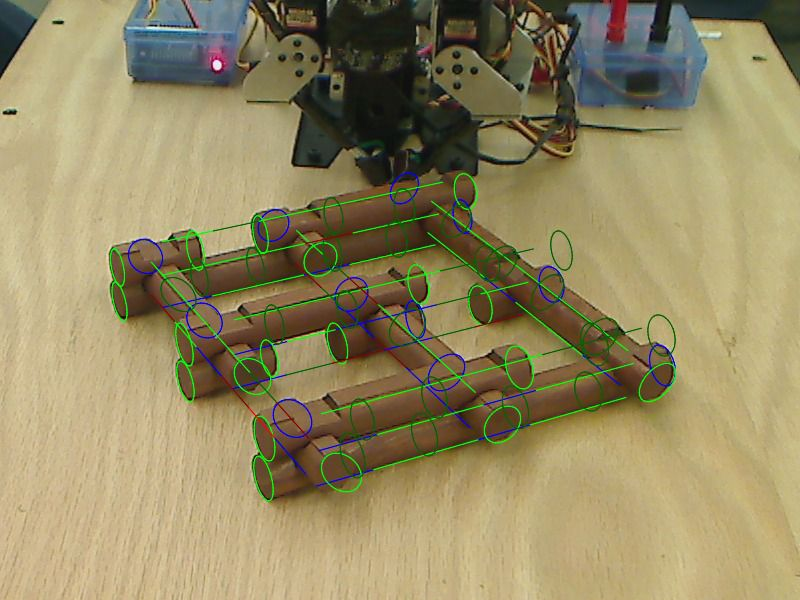
\includegraphics[width=0.195\textwidth]{images/1263244624-1500-0-end.jpg}&
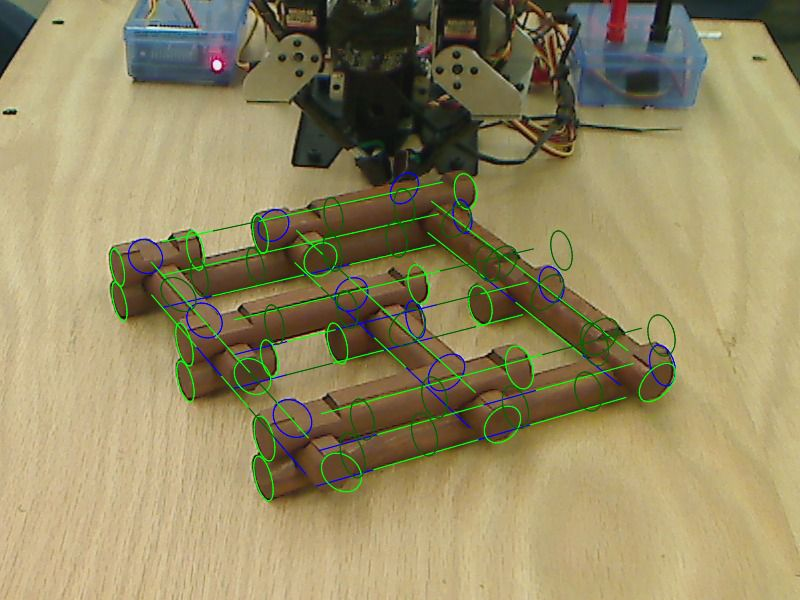
\includegraphics[width=0.195\textwidth]{images/1263244624-1500-0-both.jpg}&
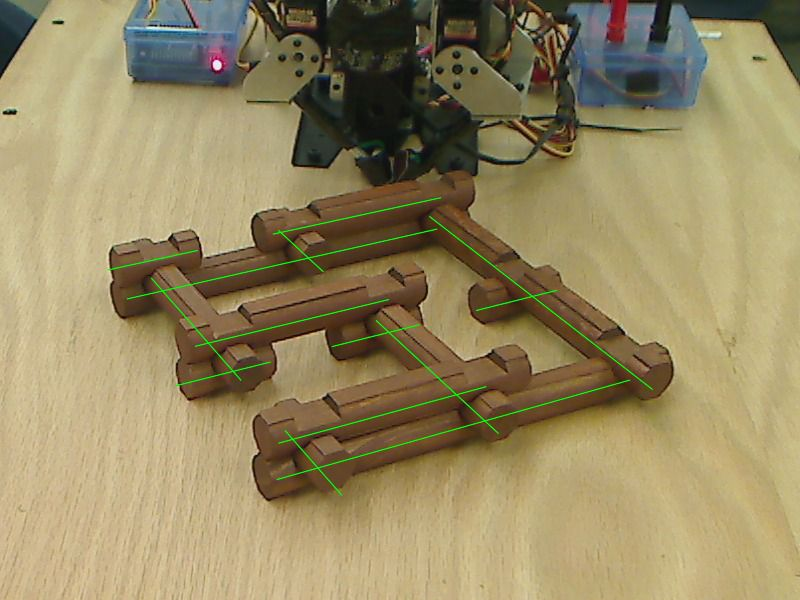
\includegraphics[width=0.195\textwidth]{images/1263244624-1500-0.jpg}\\[-0.7ex]
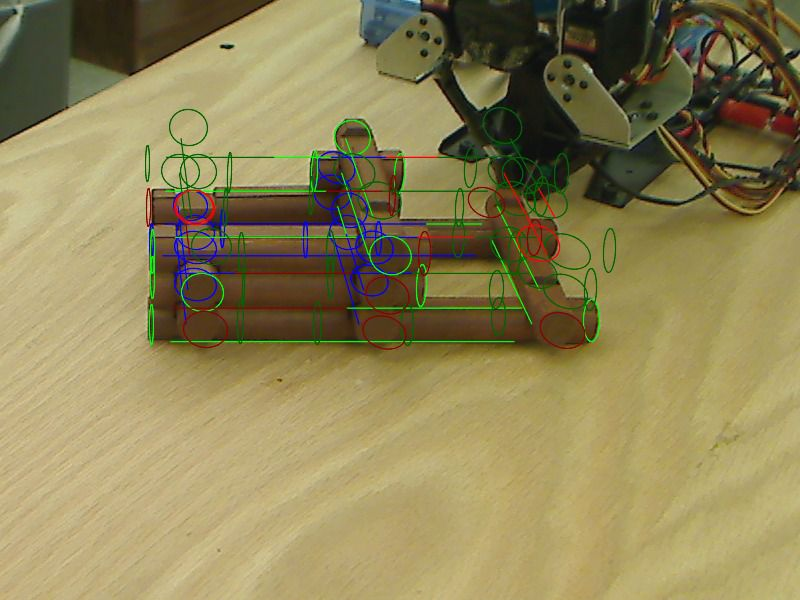
\includegraphics[width=0.195\textwidth]{images/1263244065-1200-ll-raw.jpg}&
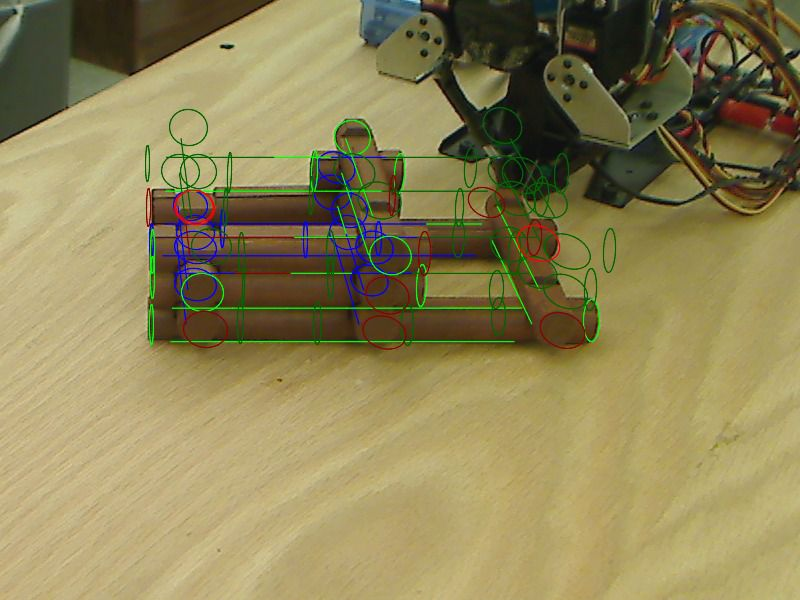
\includegraphics[width=0.195\textwidth]{images/1263244065-1200-ll-segment.jpg}&
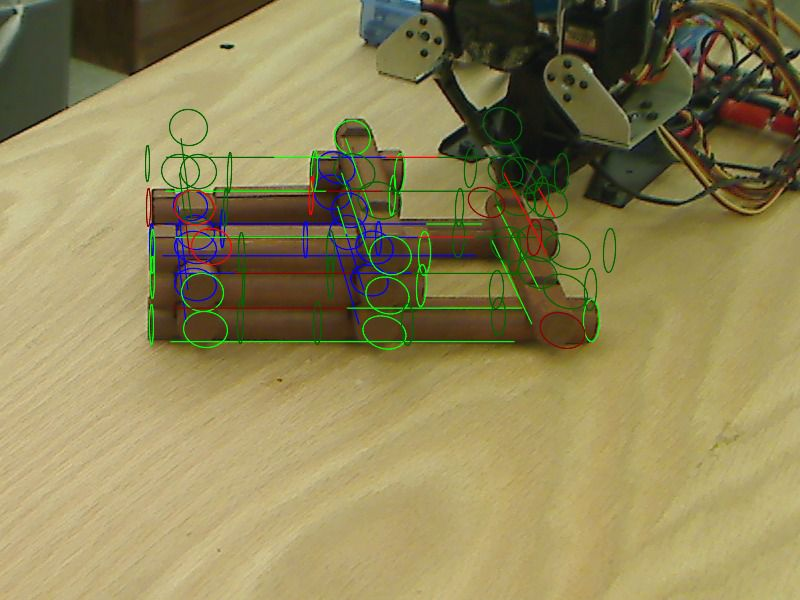
\includegraphics[width=0.195\textwidth]{images/1263244065-1200-ll-end.jpg}&
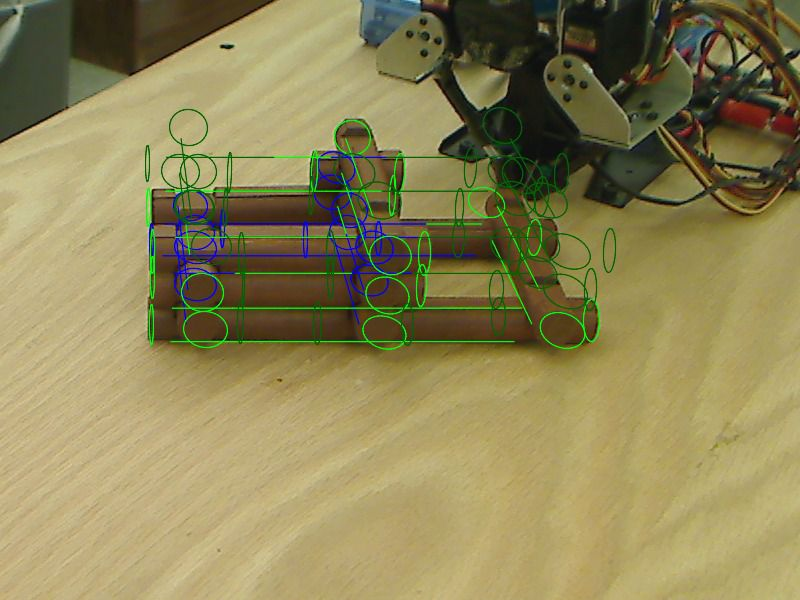
\includegraphics[width=0.195\textwidth]{images/1263244065-1200-ll-both.jpg}&
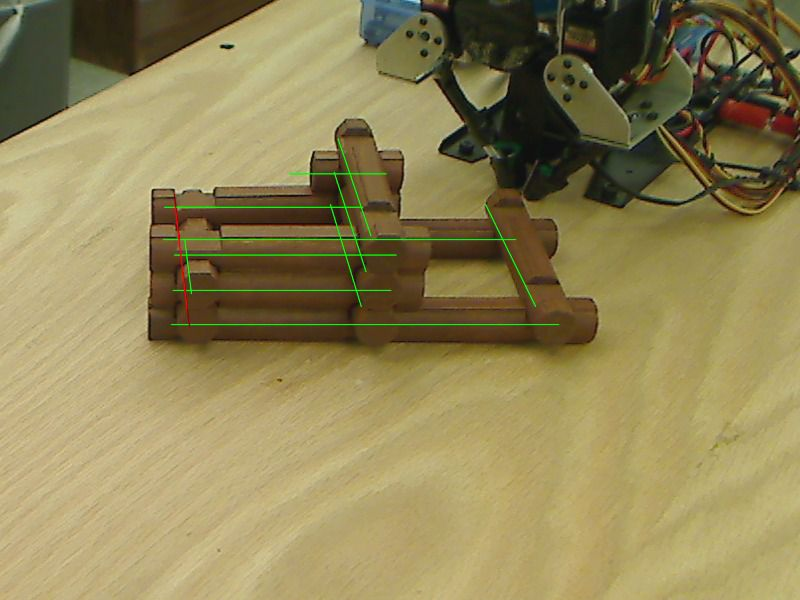
\includegraphics[width=0.195\textwidth]{images/1263244065-1200-ll.jpg}\\[-0.7ex]
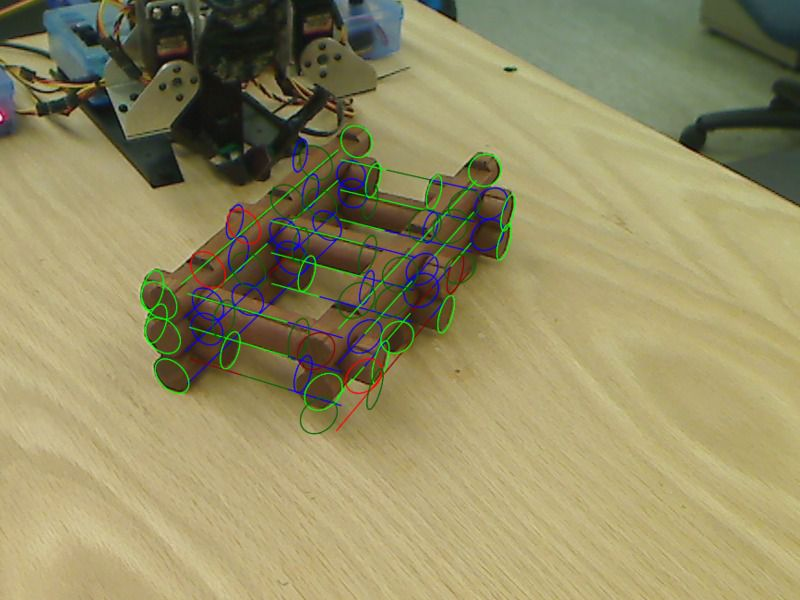
\includegraphics[width=0.195\textwidth]{images/1263242135-1800-ll-raw.jpg}&
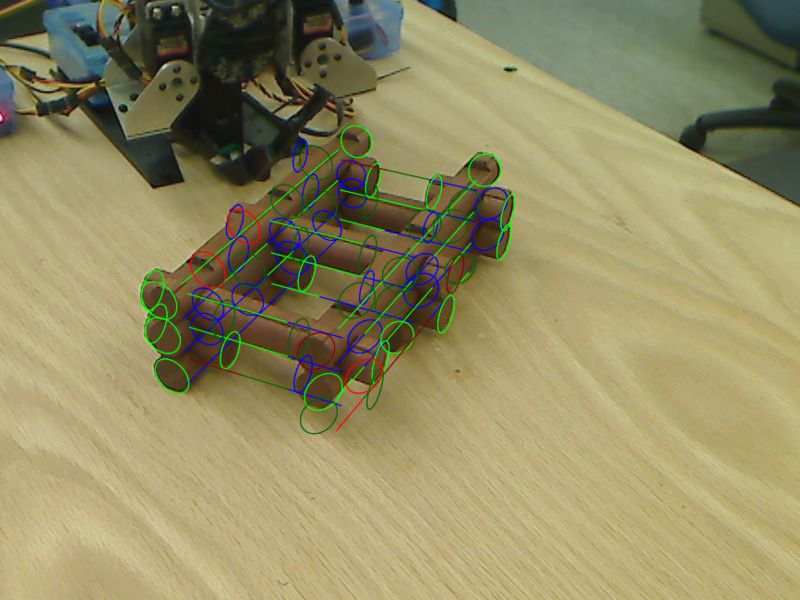
\includegraphics[width=0.195\textwidth]{images/1263242135-1800-ll-segment.jpg}&
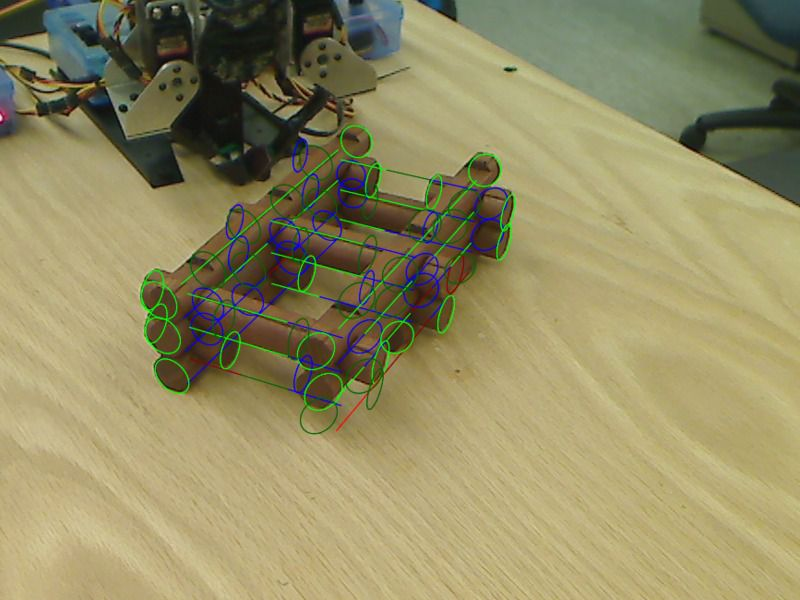
\includegraphics[width=0.195\textwidth]{images/1263242135-1800-ll-end.jpg}&
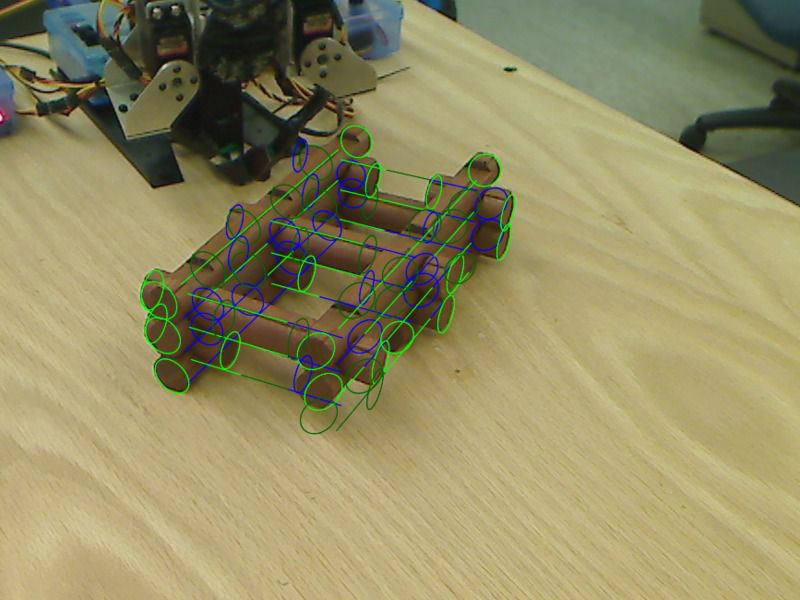
\includegraphics[width=0.195\textwidth]{images/1263242135-1800-ll-both.jpg}&
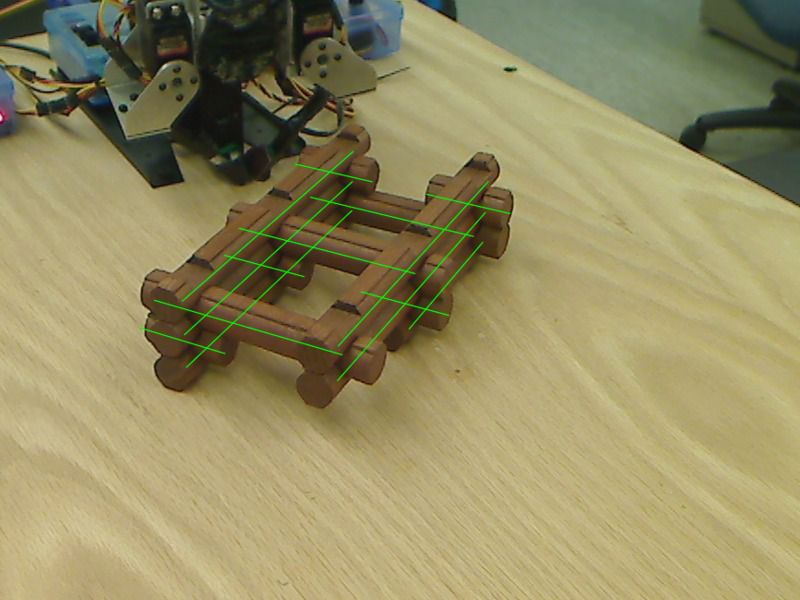
\includegraphics[width=0.195\textwidth]{images/1263242135-1800-ll.jpg}\\[-0.7ex]
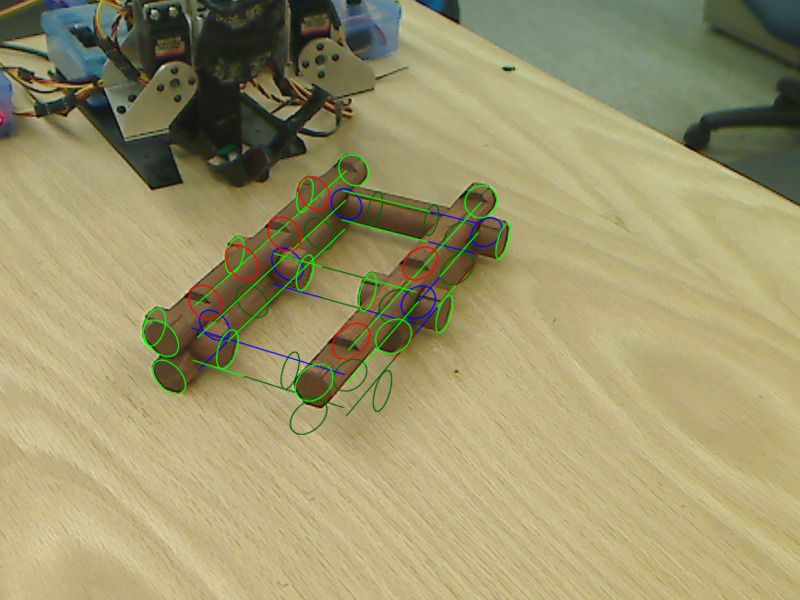
\includegraphics[width=0.195\textwidth]{images/1263242360-1800-0-raw.jpg}&
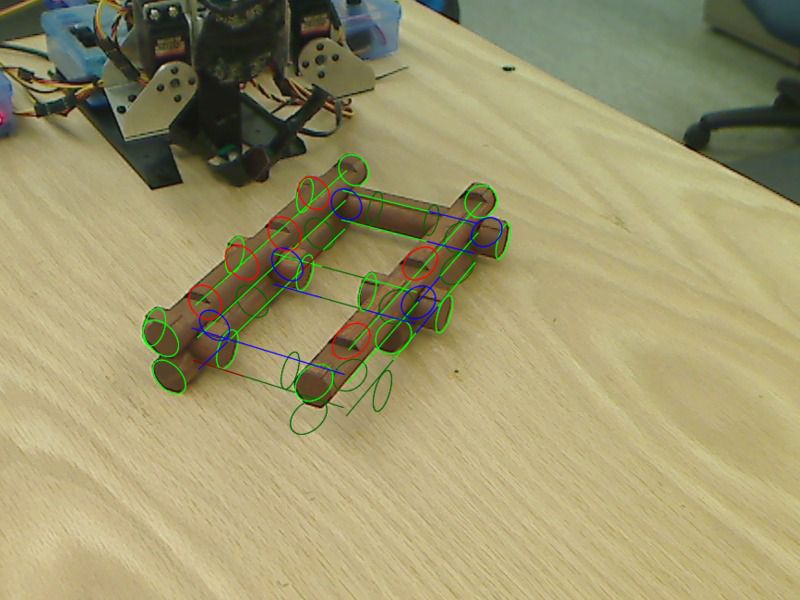
\includegraphics[width=0.195\textwidth]{images/1263242360-1800-0-segment.jpg}&
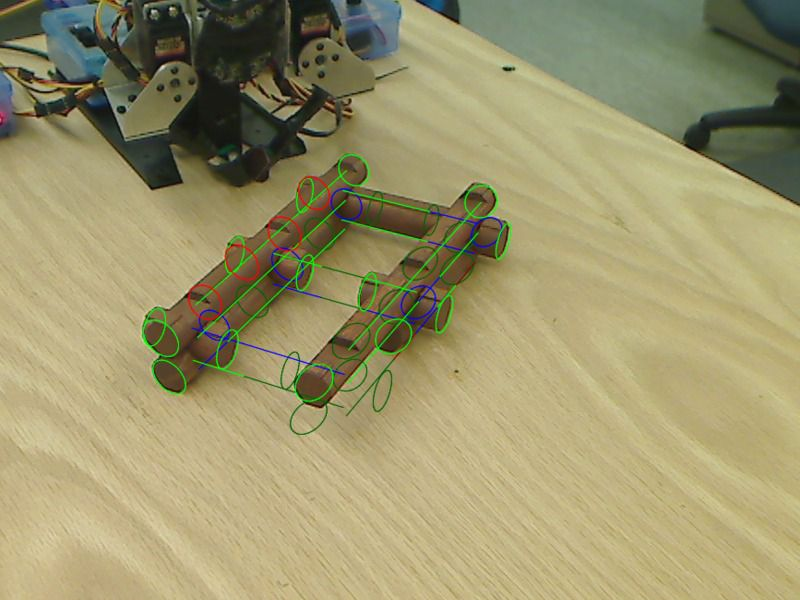
\includegraphics[width=0.195\textwidth]{images/1263242360-1800-0-end.jpg}&
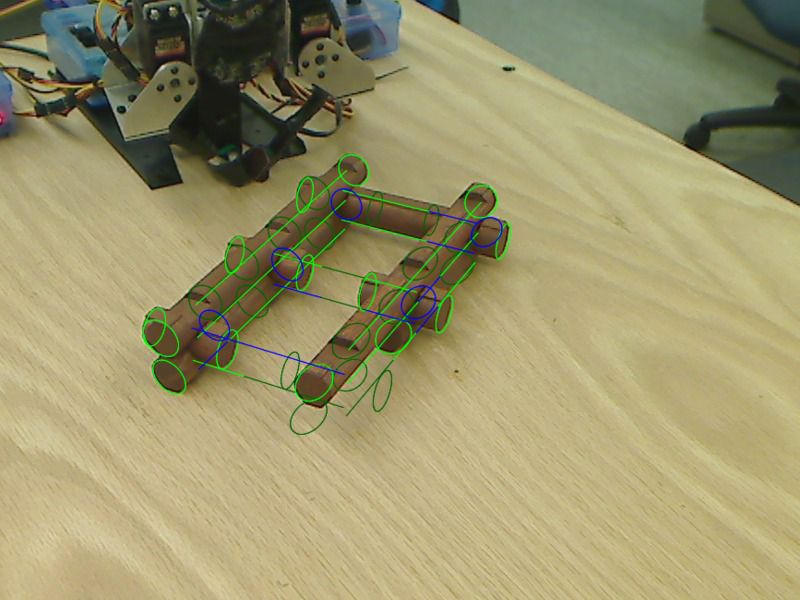
\includegraphics[width=0.195\textwidth]{images/1263242360-1800-0-both.jpg}&
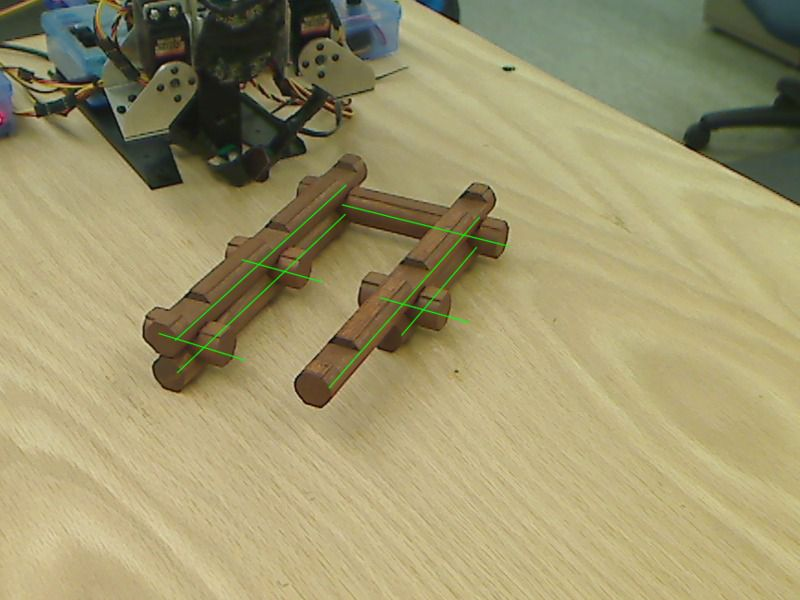
\includegraphics[width=0.195\textwidth]{images/1263242360-1800-0.jpg}\\[-0.7ex]
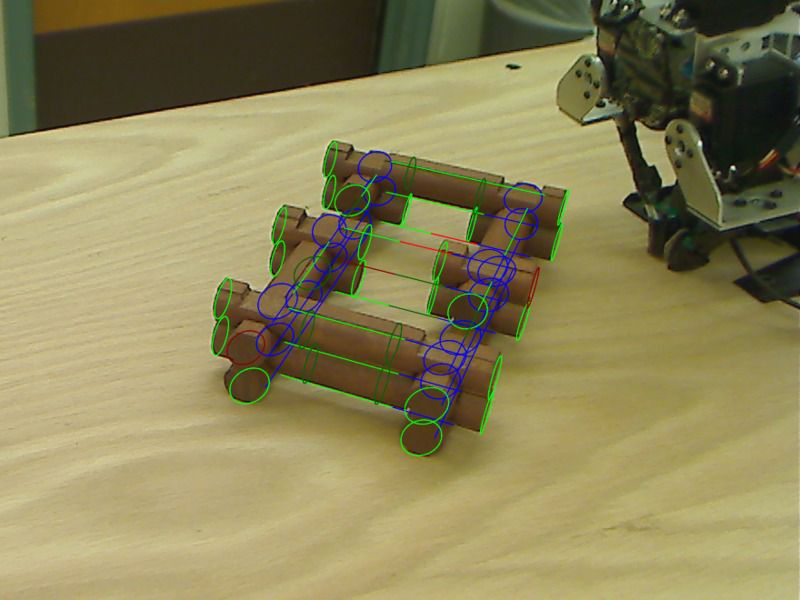
\includegraphics[width=0.195\textwidth]{images/1263243842-900-0-raw.jpg}&
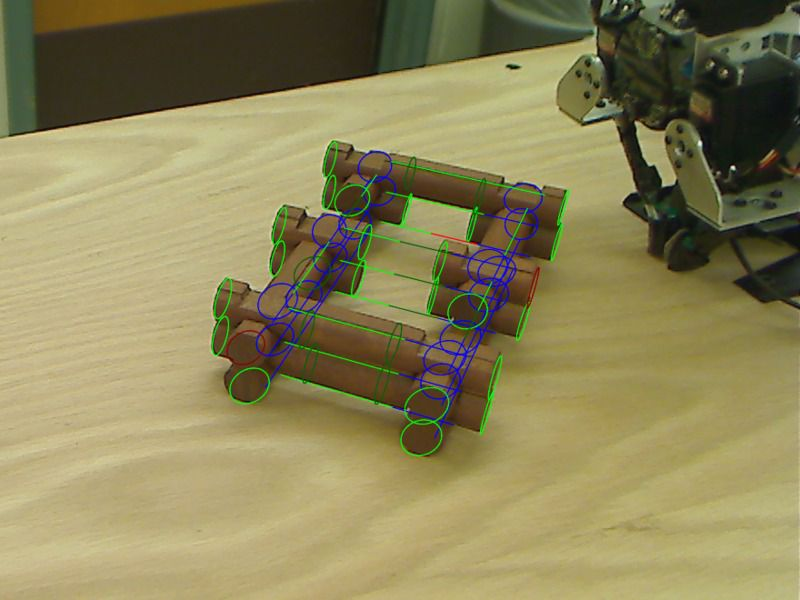
\includegraphics[width=0.195\textwidth]{images/1263243842-900-0-segment.jpg}&
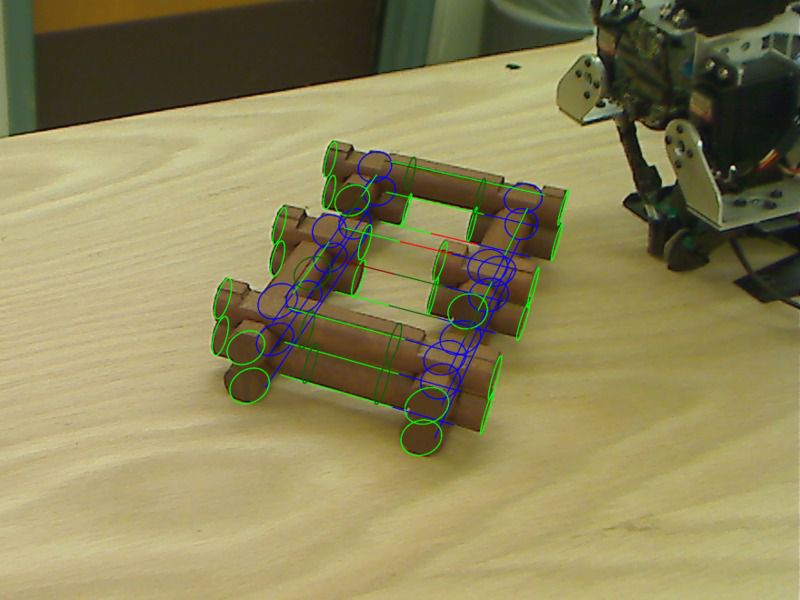
\includegraphics[width=0.195\textwidth]{images/1263243842-900-0-end.jpg}&
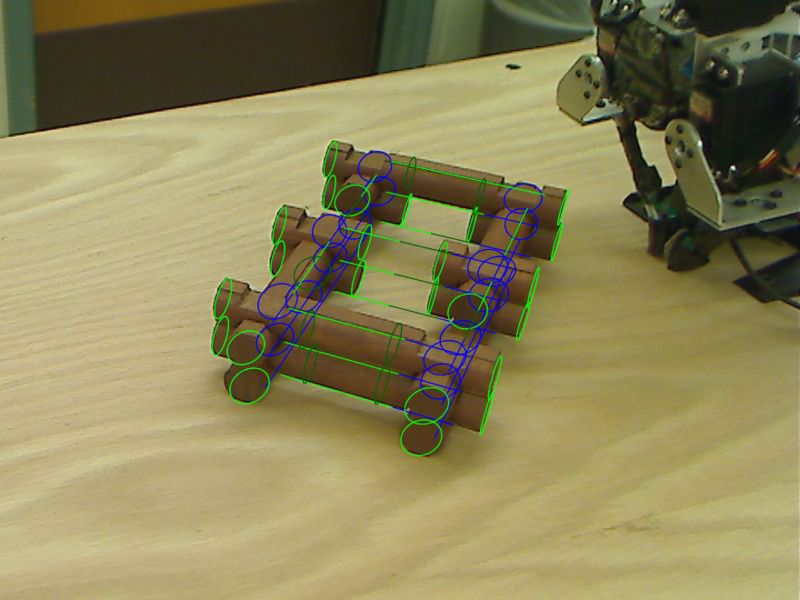
\includegraphics[width=0.195\textwidth]{images/1263243842-900-0-both.jpg}&
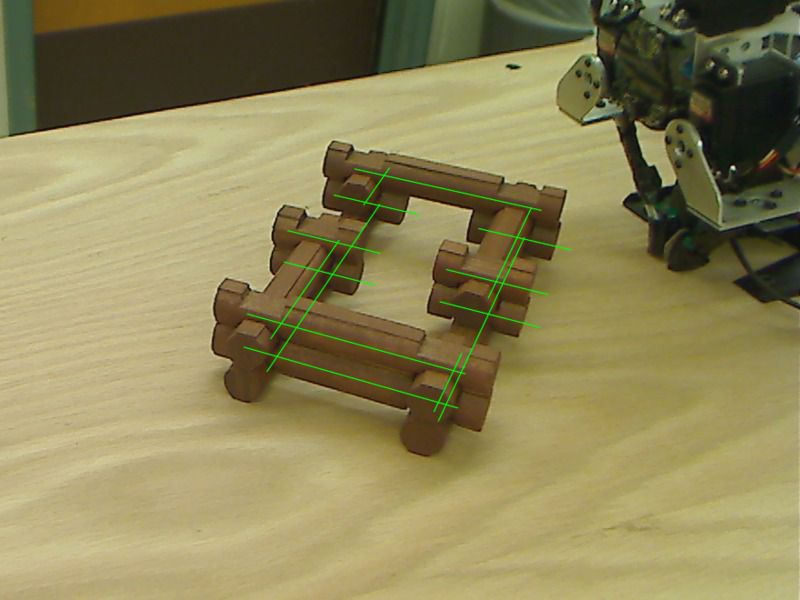
\includegraphics[width=0.195\textwidth]{images/1263243842-900-0.jpg}\\
(a)&(b)&(c)&(d)&(e)
\end{tabular}
%
\caption{\small (a)~Raw detector response.
%
(b)~Detector response with just constraints
  \ref{constraintA}--\ref{constraintD} and
  \ref{constraintF}--\ref{constraintG}.
%
(c)~Detector response with just constraints
  \ref{constraintA}--\ref{constraintE}.
%
(d)~Detector response with all constraints.
%
(e)~Estimated structure.
%
In~(a--d), bright red indicates true negative, dark red indicates false
negative, bright green indicates true positive, dark green indicates false
positive, and blue indicates occlusion.
%
In~(e), green indicates true positive and red indicates false negative.
%
There are no false positives and true negatives are not indicated.
%
We suggest that the reader view this figure at a high magnification level in a
PDF viewer to appreciate the images.
}
%
\label{fig-ll1:results}
\end{figure}

We took images of~32 distinct \LincolnLog\ structures, each from~5 distinct
poses resulting in a total of~160 images.
%
We performed foreground-background separation and pose estimation for all~160
images using the methods from section~\ref{sec-ll1:pose}.
%
Pose was estimated within~5mm translation and~2$^{\circ}$ rotation of ground
truth for~142 images.
%
We discarded the~18 images with inaccurate pose estimation and performed
structure estimation on the remainder.
%
The results for~5 images, all of distinct structures, are shown in
Fig.~\ref{fig-ll1:results}.
%
Fig.~\ref{fig-ll1:results}(a) was derived by thresholding the priors on~$Z^+_q$,
$Z^-_q$, $Z^u_q$, $Z^v_q$, and~$Z^w_q$ at $t=0.5$.
%
Fig.~\ref{fig-ll1:results}(b--d) were derived by solving a stochastic CSP with
various subsets of the constraints and rendering the values of~$Z^+_q$,
$Z^-_q$, $Z^u_q$, $Z^v_q$, and~$Z^w_q$ for the solution provided by the first
method in section~\ref{sec-ll1:structure}.
%
Fig.~\ref{fig-ll1:results}(e) was derived by solving the stochastic CSP with all
constraints and rendering the values of~$Z_q$ for the solution provided by the
first method in section~\ref{sec-ll1:structure}.
%
Note that our method determines the correct component type ($Z_q$) of most
occluded logs in the assemblies in the second row of Fig.~\ref{fig-ll1:results}(e).
%
It gives an incorrect component type for only a single log in that row.

We conducted experiments to determine how much the grammar improves the
accuracy of structure estimation.
%
We performed variants of the runs in Fig.~\ref{fig-ll1:results}(a-d), varying the
threshold~$t$ and the mapping from evidence to priors to produce the ROC curves
depicted in Fig.~\ref{fig-ll1:roc}.
%
The mapping function is varied through the weighting factor~$e$ for the linear
interpolator discussed in section~\ref{sec-ll1:mapping}.

Pose and structure estimation is sufficiently robust to support robotic
manipulation.
%
Supplementary material included on the website for this paper contains videos
of fully autonomous robotic disassembly of six different \LincolnLog\
structures whose pose and structure have been determined from a single image as
well as videos of semiautonomous robotic assembly of replicate \LincolnLog\
structures from the same estimated pose and structure.

\section{Conclusion}
\label{sec-ll1:conclusion}

\LincolnLogs\ are children's toys yet the computational problem we present is
\emph{not} a toy.
%
Pose and structure estimation of \LincolnLog\ assemblies is \emph{far} more
difficult than may appear on the surface.
%
The space of objects to be recognized is combinatorially large.
%
Much of every structure is in self occlusion.
%
The low contrast due to shadows and color, intensity, and texture uniformity
make it impossible to recognize even \emph{visible} logs with existing
techniques.
%
No standard edge detector (\eg\ Canny \cite{Canny1986} or \Pb\
\cite{Maire2008}) can reliably find edges separating adjacent logs or circular
log ends and no standard segmentation method (\eg\ Normalized Cut
\cite{Shi2000} or Mean Shift \cite{Comaniciu2002}) can reliably find log parts
\emph{even when fully visible} as shown in Fig.~\ref{fig-ll1:comparison}.
%
Even our filter-based feature detectors, which use pose information along with
constraints from the language model to \emph{tune to the expected feature at
  the expected image position}, produce correct binary decisions only about
65\% of the time.
%
Occlusion only makes matters worse.
%
Performing non-stochastic constraint satisfaction (\eg\ Waltz line labeling
\cite{Waltz1975}) on the binary output of these detectors leads to
inconsistent CSPs on \emph{all} images in our dataset.

We have demonstrated a visual domain that is generative in much the same way
that human language is generative.
%
We have presented a visual language model that improves recognition accuracy in
this domain in much the same way that language models improve
speech-recognition accuracy.
%
Unlike context-free models of human language, our visual language models are
context sensitive and formulated as stochastic CSPs.
%
Much of our visual experience in the artifactual world is perceiving generative
man-made structures like buildings, furniture, vehicles, \etc{}
%
Our \LincolnLog\ domain is a first step towards building visual language models
for such real-world domains.

Language models for vision are more complex than those for human language as
they must deal with occlusion resulting from perspective projection and pose
variation.
%
However, visual domains exhibit a novel possibility: recovering structure
despite occlusion by integrating the perceptual evidence from multiple images
of the same object taken from different poses.
%
In the \LincolnLog\ domain, one can carry this even further.
%
When faced with ambiguity arising from occlusion, a robot can partially
disassemble a structure to view occluded substructure and integrate perceptual
evidence from multiple images taken at different disassembly stages to yield a
complete unambiguous estimate of the structure of the original assembly prior
to disassembly.
%
Moreover, it is possible to integrate information about pose or structure from
different modalities.
%
One can integrate partial pose and structure information from one or more
images with partial pose and structure information expressed in human language
to yield a complete unambiguous estimate of pose and structure.
%
We are, in fact, able to do this and expect to report on this in the future.
